\documentclass[10pt,fleqn]{article}
%\usepackage[journal=rsc]{chemstyle}
%\usepackage{mhchem}
\usepackage{amsmath}
\usepackage{amssymb}
\usepackage{amsfonts}
\usepackage{esint}
\usepackage{bbm}
\usepackage{amscd}
\usepackage{picinpar}
\usepackage[pdftex]{graphicx}
\usepackage{indentfirst}
\usepackage{wrapfig}
\usepackage{units}
\usepackage{textcomp}
\usepackage[utf8x]{inputenc}
\usepackage{feyn}
\usepackage{feynmp}
\usepackage{listings}
\DeclareGraphicsRule{*}{mps}{*}{}
\newcommand{\ud}{\mathrm{d}}
\newcommand{\ue}{\mathrm{e}}
\newcommand{\ui}{\mathrm{i}}
\newcommand{\res}{\mathrm{Res}}
\newcommand{\Tr}{\mathrm{Tr}}
\newcommand{\dsum}{\displaystyle\sum}
\newcommand{\dprod}{\displaystyle\prod}
\newcommand{\dlim}{\displaystyle\lim}
\newcommand{\dint}{\displaystyle\int}
\newcommand{\fsno}[1]{{\!\not\!{#1}}}
\newcommand{\eqar}[1]
{
  \begin{align*}
    #1
  \end{align*}
}
\newcommand{\texp}[2]{\ensuremath{{#1}\times10^{#2}}}
\newcommand{\dexp}[2]{\ensuremath{{#1}\cdot10^{#2}}}
\newcommand{\eval}[2]{{\left.{#1}\right|_{#2}}}
\newcommand{\paren}[1]{{\left({#1}\right)}}
\newcommand{\lparen}[1]{{\left({#1}\right.}}
\newcommand{\rparen}[1]{{\left.{#1}\right)}}
\newcommand{\abs}[1]{{\left|{#1}\right|}}
\newcommand{\sqr}[1]{{\left[{#1}\right]}}
\newcommand{\crly}[1]{{\left\{{#1}\right\}}}
\newcommand{\angl}[1]{{\left\langle{#1}\right\rangle}}
\newcommand{\tpdiff}[4][{}]{{\paren{\frac{\partial^{#1} {#2}}{\partial {#3}{}^{#1}}}_{#4}}}
\newcommand{\tpsdiff}[4][{}]{{\paren{\frac{\partial^{#1}}{\partial {#3}{}^{#1}}{#2}}_{#4}}}
\newcommand{\pdiff}[3][{}]{{\frac{\partial^{#1} {#2}}{\partial {#3}{}^{#1}}}}
\newcommand{\diff}[3][{}]{{\frac{\ud^{#1} {#2}}{\ud {#3}{}^{#1}}}}
\newcommand{\psdiff}[3][{}]{{\frac{\partial^{#1}}{\partial {#3}{}^{#1}} {#2}}}
\newcommand{\sdiff}[3][{}]{{\frac{\ud^{#1}}{\ud {#3}{}^{#1}} {#2}}}
\newcommand{\tpddiff}[4][{}]{{\left(\dfrac{\partial^{#1} {#2}}{\partial {#3}{}^{#1}}\right)_{#4}}}
\newcommand{\tpsddiff}[4][{}]{{\paren{\dfrac{\partial^{#1}}{\partial {#3}{}^{#1}}{#2}}_{#4}}}
\newcommand{\pddiff}[3][{}]{{\dfrac{\partial^{#1} {#2}}{\partial {#3}{}^{#1}}}}
\newcommand{\ddiff}[3][{}]{{\dfrac{\ud^{#1} {#2}}{\ud {#3}{}^{#1}}}}
\newcommand{\psddiff}[3][{}]{{\frac{\partial^{#1}}{\partial{}^{#1} {#3}} {#2}}}
\newcommand{\sddiff}[3][{}]{{\frac{\ud^{#1}}{\ud {#3}{}^{#1}} {#2}}}
\usepackage{fancyhdr}
\usepackage{multirow}
\usepackage{fontenc}
%\usepackage{tipa}
\usepackage{ulem}
\usepackage{color}
\usepackage{cancel}
\newcommand{\hcancel}[2][black]{\setbox0=\hbox{#2}%
\rlap{\raisebox{.45\ht0}{\textcolor{#1}{\rule{\wd0}{1pt}}}}#2}
\pagestyle{fancy}
\setlength{\headheight}{67pt}
\fancyhead{}
\fancyfoot{}
\fancyfoot[C]{\thepage}
\fancyhead[R]{}
\renewcommand{\footruleskip}{0pt}
\renewcommand{\headrulewidth}{0.4pt}
\renewcommand{\footrulewidth}{0pt}
\addtolength{\hoffset}{-1.3cm}
\addtolength{\voffset}{-2cm}
\addtolength{\textwidth}{3cm}
\addtolength{\textheight}{2.5cm}
\renewcommand{\footskip}{10pt}
\setlength{\headwidth}{\textwidth}
\setlength{\headsep}{20pt}
\setlength{\marginparwidth}{0pt}
\parindent=0pt
\title{Deterministic dimension independent mesh generation}
\begin{document}

\maketitle

\section{Design}

In this section, we describe the basic design of the meshing algorithm.

\subsection{Requirements}

When using finite element method, one usually use an adaptive variable size
discretization of the space in order to handle different geometries with
different precision requirement. This is very important in order to avoid
using the highest grid resolution for the whole problem and to reduce the
size of the final linear system to solve. In order to support this, we would
like our meshing algorithm to handle arbitrary geometry constraint with
arbitrary spacially varying meshing density. Since separate space can be
descretized independently, we can assume the space is connected. However, it is
not restricted to be singly connected in order to support problems with inner
surfaces.\\

In additional to these basic requirements, we would like to handle meshing
of curved space with the same algorithm. This is useful to solve problems on
a geometry embedded in a higher dimensional space, e.g. a curved surface in
three-dimensional space.

\subsection{Abstraction of the model}

In order to generate a mesh, it is necessary to specify the problem first.
Although we would like to handle arbitrary configurations mentioned in the
previous section, we do not want to write specialized code for each problems.
Therefore, before being able to generate the mesh, we first need a standardized
interface to specify the properties of the problem. The interface needs to be
flexible enough to cover different kinds of problems and it should also provide
enough information to fully specify the problem. Moreover, the information
provided by the interface should be relatively easy to generate during the
construction of the problem and it should also be easy for the meshing
algorithm to process.\\

Due to the flexible requirement, we decided that the most important properties
of the space is the constraint of allowed values (when the problem is embedded
in a higher dimensional space) and the relation between different elements.
These informations are important to make sure that the mesh we generate is
an accurate description of the problem and is not over sampling the space.
Therefore, in additional to the interfaces that provide basic informations
(e.g. problem dimension, local mesh density) we define the following two
functions to specify how to find the next point in the problem space from
the current point, and if a new mesh element is intersecting with existing
ones.

\begin{lstlisting}
    get_next_point{N,V}(model::AbstractModel{N,V}, point::V,
                        step::V, section::Int, clip::Bool)
    check_crossing{N,V}(model::AbstractModel{N,V}, orig_points::NTuple{N,V},
                        point2::V, tileset::TileSet{N,V})
\end{lstlisting}

With a reasonably small grid size and slow variation of space parameters, these
informations can be determined from only local informations of the model and
are therefore easy to generate.

\section{Implementation}

In this section, we describe our implementation of the algorithm. We do not
cover all the technical detail about the implementation, which can be more
clearly explained by the code itself. Instead, we will describe the important
steps in the algorithm and a breif outline how they are implemented.\\

Since our abstraction of the model only contain local information of the space,
the algorithm we use to generate the mesh is naturally an iterative method
that covers the whole space by locally extending the current mesh. In each
iteration, we pick an edge/surface we previously generateed and try to construct
the next one out of it. When generating it, in additional to making sure we are
using the right grid size, we also need to make sure that it is within the valid
region and does not cross with existing ones. In order to do this, we use the
following steps,

\begin{itemize}
\item Check if the current point is close enough to the boundary.

  If it is closer than a certain threshold ($10\%$ of the grid size), we
  simply treat it as a point on the boundary and do not extend it.

\item Determine if we should simply combine with a neighbering edge.

  In order to do this, we check all of the mesh elements that are directly
  connected and check if the angle between the two is suitable for generating
  the next element.

\item Look for other existing mesh elements nearby.

  If there are any other nearby elements that are not directly connected with
  the current one, we pick one of the point among them to construct the next
  element. We look for nearby elements by calculating the distance from each
  element to a certain point near or on the current element and therefore
  does not require any interaction with the model itself. This is a
  generalization of the previous step but requires more arithmetics and is
  more expensive.

\item Now we can add a new mesh element independent of other ones.

  The only thing we still need to be careful about is the boundary of the
  area, which is handled by the check\_crossing function.
\end{itemize}

During this process, we keep track of the new elements addes and in which
directions they should be extended. We terminate the iteration when there is
no element left to be extended and the whole space is covered.

\section{Results}

Due to time constraint, we have only implemented and debugged the meshing
algorithm for one and two dimensional systems. However, we could demonstrate
that the algorithm works unmodified for meshing a curved space embedded in a
higher dimention, for example, the edge of a circle or the surface of a sphere.
We also demonstrated that we can use post-generation optimization passes to
improve the homogeneity of the mesh.

\subsection{Meshing the edge of a circle}

\begin{center}
  \includegraphics[width=8cm]{../MeshGen/img/mesh1d.png}
\end{center}

The coordinates are expressed directly with a two dimensional vector instead
of a single number and the algorithm can handle this very well. We can also see
the variation of the meshing density follows what we specified.

\subsection{Meshing a circle with a hole and variable density}

\begin{center}
  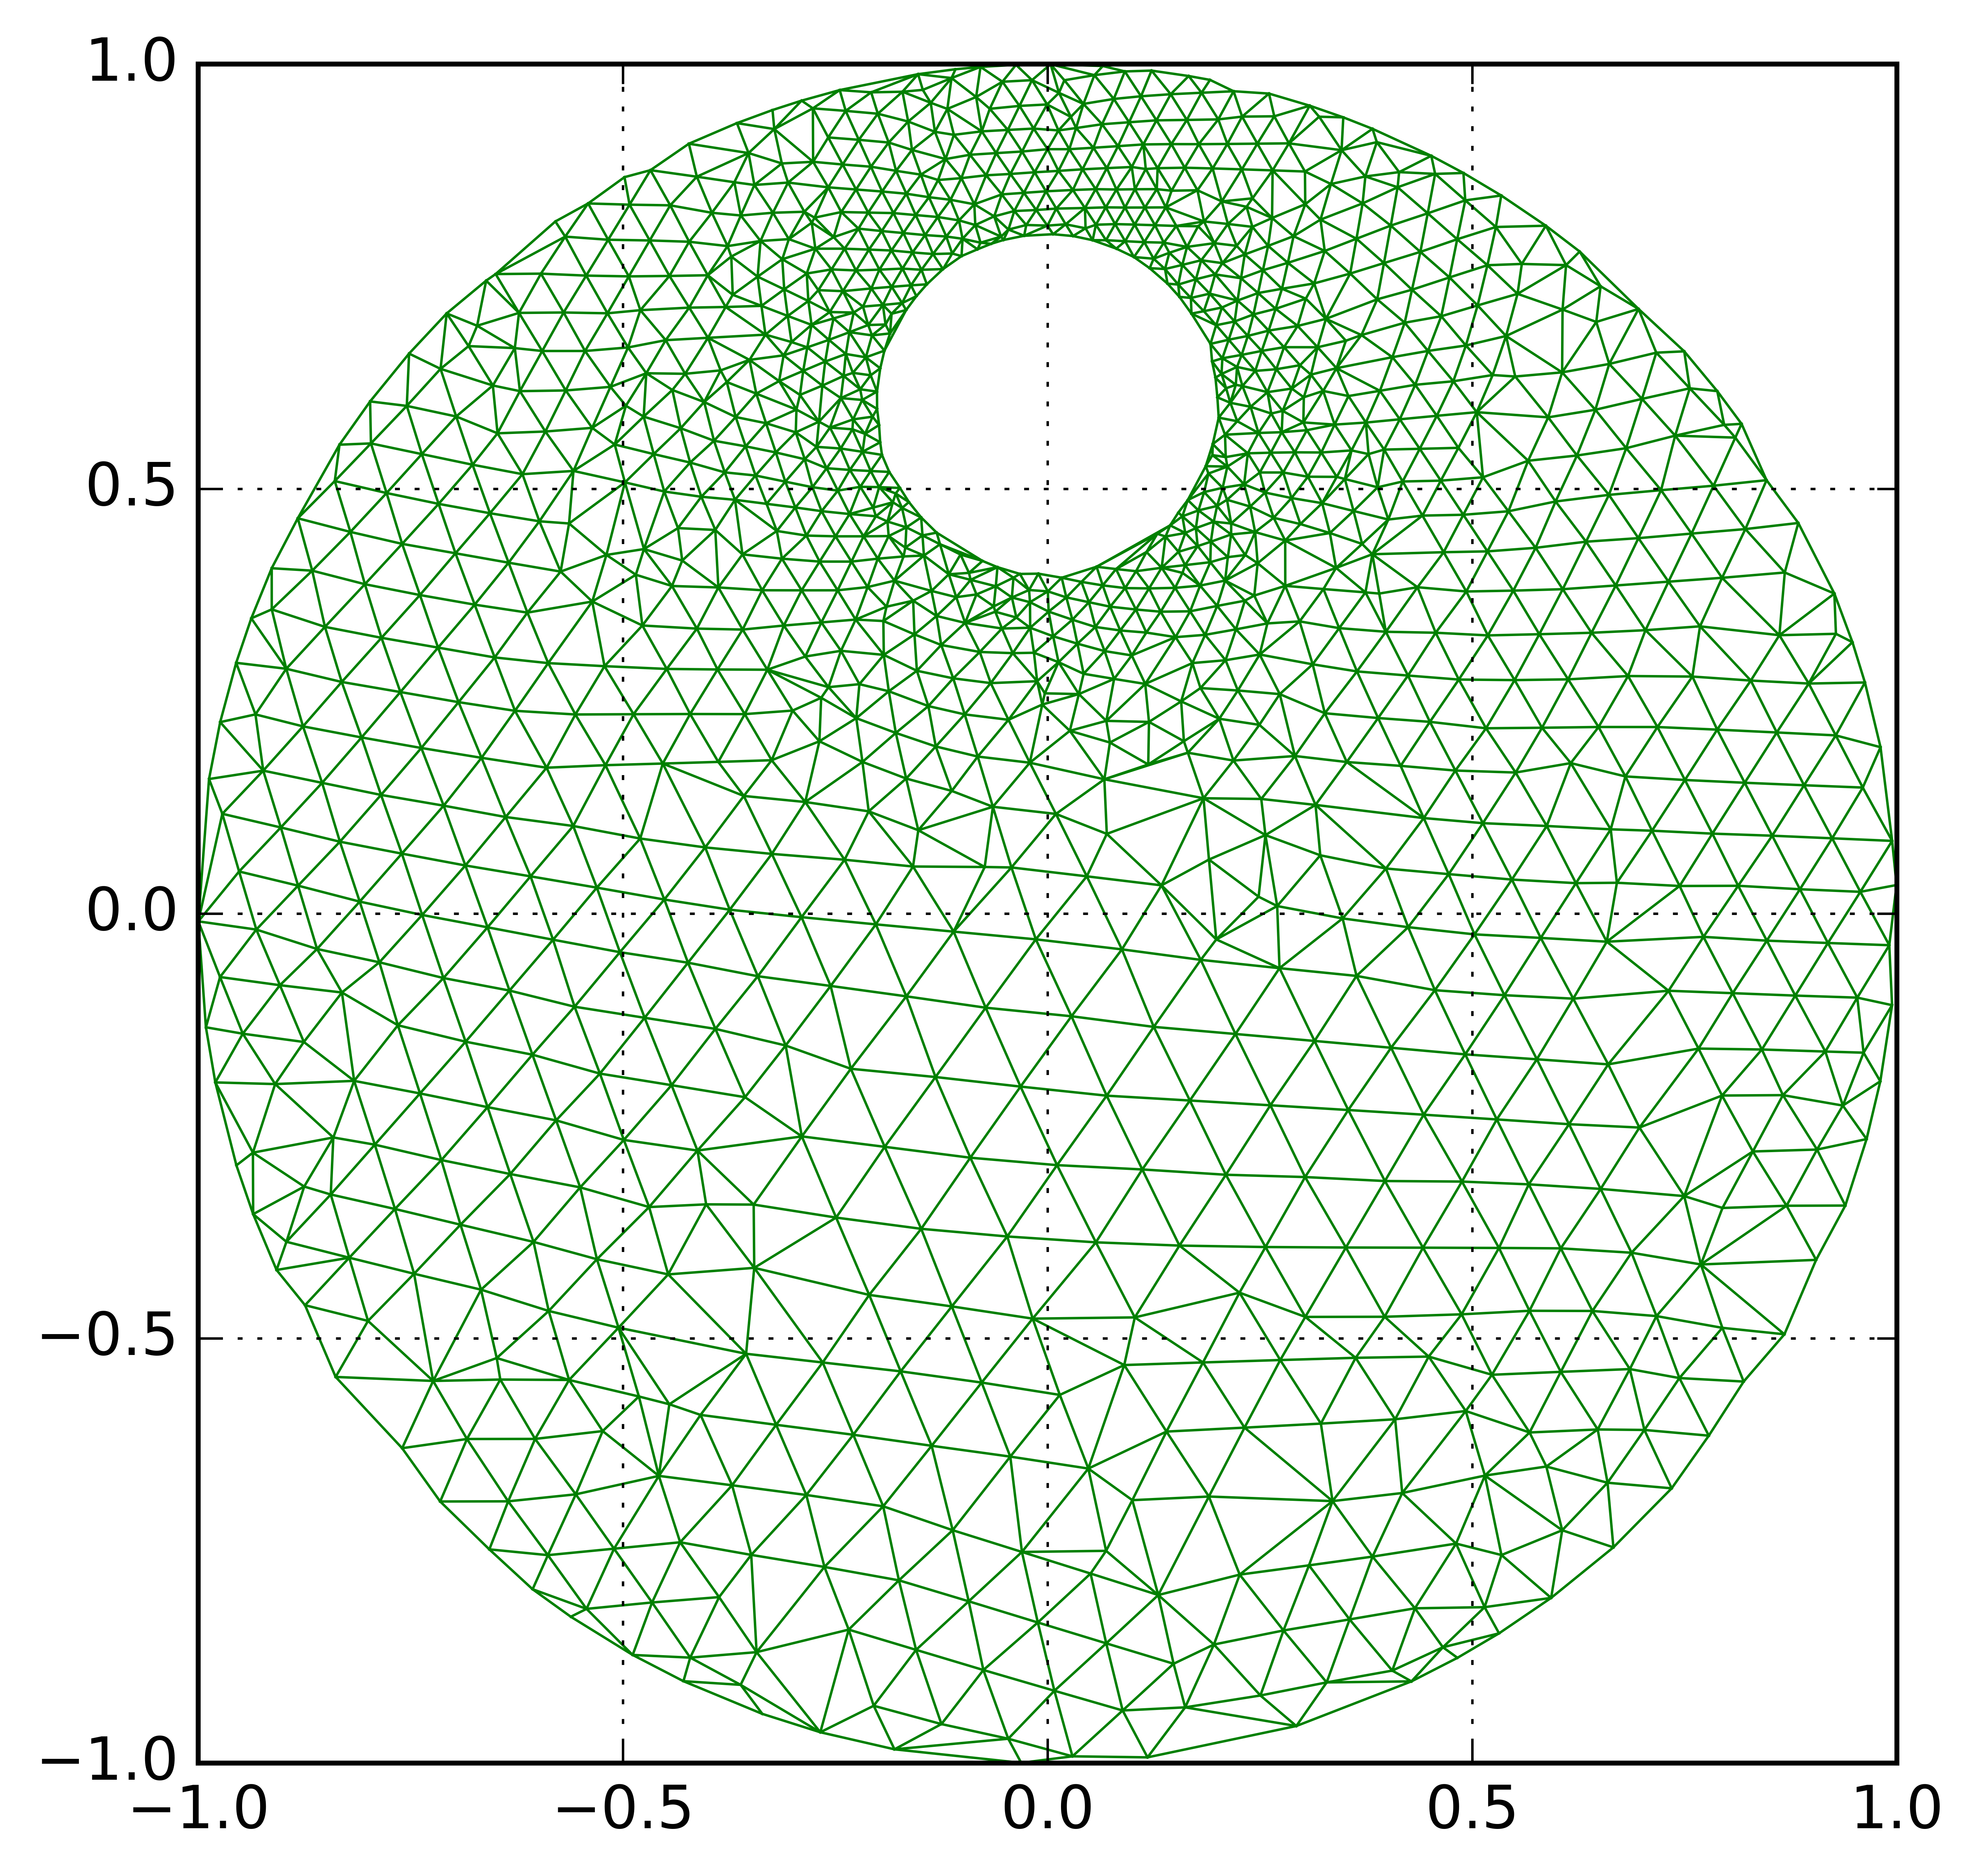
\includegraphics[width=8cm]{../MeshGen/img/mesh2d_circ.png}
\end{center}

The algorithm smoothly connect the region near the hole with higher meshing
density to the region near the center with lower density. It also correctly
avoided the hole during the meshing process.

\subsection{Post meshing optimization}

\begin{center}
  \includegraphics[width=6cm]{../MeshGen/img/mesh2d_circ_noopt.png}
  \includegraphics[width=6cm]{../MeshGen/img/mesh2d_circ_opt.png}\\
\end{center}

Here we show a part of the mesh before and after we apply the optimization pass.
We clearly see that by rearranging the connection, we could remove many thin
and unevenly sided triangles we generate.

\subsection{Meshing a three dimenstional curved surface}

\begin{center}
  \includegraphics[width=7cm]{../MeshGen/img/mesh2d_sphere_front.png}
  \includegraphics[width=7cm]{../MeshGen/img/mesh2d_sphere_back.png}
\end{center}

This is the result of meshing the surface of a sphere in three dimenstion using
the same algorithm. The plot shows the projection of the mesh in the front and
back side of the sphere onto a two dimensional plane. The mesh spacing are
smaller closed to the edge of the edge because of the projection.

\section{Future improvements}

\end{document}
